\documentclass[12pt]{article}
\usepackage[T1]{fontenc}
\usepackage[utf8]{inputenc}
\usepackage{polski}
\usepackage{minted}
\usepackage{geometry}
\usepackage{natbib}
\usepackage{enumitem}
\usepackage{graphicx}
\usepackage{bold-extra}
\usepackage[font=small,labelfont=bf]{caption}
\usepackage{hyperref}
\usepackage{titlesec}
\usepackage{indentfirst}
\hyphenpenalty=10000
\tolerance=1000 \emergencystretch=2em
\titlelabel{\thetitle.\quad}

 \geometry{
     left=23mm,
     top=25mm,
     right=23mm
 }


\def\mydate{\leavevmode\hbox{\twodigits\day.\twodigits\month.\the\year}}
\def\twodigits#1{\ifnum#1<10 0\fi\the#1}

\begin{document}
%titlepage
\thispagestyle{empty}
\begin{center}
\begin{minipage}{0.75\linewidth}
    \centering
    
\includegraphics[width=0.45\linewidth]{agh_logo2.png}
    \par
    \vspace{2cm}
    {\bfseries{\scshape{\Huge  Teoria współbieżności}}}
    \par
    \vspace{1.7cm}
    {\scshape{\Large Laboratorium 8}}
    \par
    \vspace{0.8cm}
    {\scshape{\Large Wzorce Executor i Future}}
    \par
    \vspace{3cm}

    {\scshape{\Large Albert Gierlach}}\par
    \vspace{1cm}

    {\Large \mydate}
\end{minipage}
\end{center}
\clearpage



\section{Zadanie 1}
Proszę zaimplementować przy użyciu Executor i Future program wykonujący obliczanie zbioru Mandelbrota w puli wątków.
  
\section{Koncept rozwiązania}
Do przykładowego kodu zostanie dodane wsparcie dla wielowątkowości. Jako, że pętla wewnętrzna obliczająca kolejne piksele w wierszu wynikowego obrazu nie zależy od wartości poprzednich, to możemy rozdzielić ją między wątki tak, że każdy z nich będzie obliczał jeden wiersz obrazu.


\section{Implementacja oraz wyniki}
\begin{minted}[frame=lines,
                framesep=2mm
                ]{java}
class MandelbrotWorker implements Callable<Void> {
    private final double ZOOM = 150;

    private final int iters;
    private final int w;
    private final int current_h;
    private final BufferedImage img;

    public MandelbrotWorker(int iters, int w, int current_h, BufferedImage img) {
        this.iters = iters;
        this.w = w;
        this.current_h = current_h;
        this.img = img;
    }

    @Override
    public Void call() {
        double cY = (current_h - 300) / ZOOM;
        for (int x = 0; x < w; x++) {
            double zy = 0;
            double zx = 0;
            double cX = (x - 400) / ZOOM;
            int iter = iters;
            while (zx * zx + zy * zy < 4 && iter > 0) {
                double tmp = zx * zx - zy * zy + cX;
                zy = 2.0 * zx * zy + cY;
                zx = tmp;
                iter--;
            }
            img.setRGB(x, current_h, iter | (iter << 8));
        }
        return null;
    }
}

class Mandelbrot extends JFrame {
    private final int maxIter;
    private final BufferedImage img;
    private final int width;
    private final int height;

    public Mandelbrot(int max_iter) {
        super("Mandelbrot Set");
        setBounds(100, 100, 800, 600);
        setResizable(false);
        setDefaultCloseOperation(EXIT_ON_CLOSE);

        this.maxIter = max_iter;
        this.width = getWidth();
        this.height = getHeight();
        this.img = new BufferedImage(getWidth(), height, BufferedImage.TYPE_INT_RGB);
    }

    public void run(ExecutorService executorService){
        var futures = new LinkedList<Future<Void>>();
        for (int y = 0; y < height; y++) {
            var task = new MandelbrotWorker(maxIter, width, y, img);
            futures.add(executorService.submit(task));
        }

        for(var f : futures){
            try {
                f.get();
            } catch (InterruptedException | ExecutionException e) {
                e.printStackTrace();
            }
        }
    }

    public void display(){
        setVisible(true);
    }

    @Override
    public void paint(Graphics g) {
        g.drawImage(img, 0, 0, this);
    }
}

class Main{
    public static void main(String[] args) {
        var mandelbrot = new Mandelbrot(570);
        var executor = Executors.newFixedThreadPool(4);
        mandelbrot.run(executor);
        mandelbrot.display();
    }
}
\end{minted}

\newpage
\noindent
Wykonanie programu dało następujące wyniki:
\begin{center}
\centering
    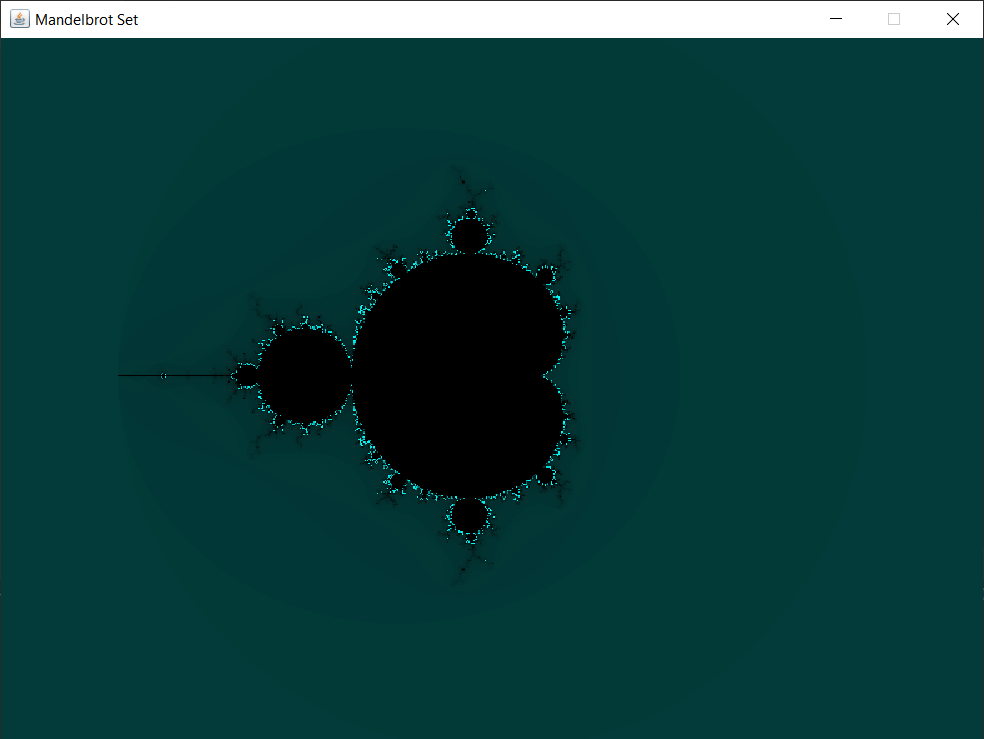
\includegraphics[scale=0.8]{mandel1.png}
    \captionof{figure}{Wynikowy zbiór Mandelbrota}
\end{center}


\section{Wnioski}
Program wygenerował poprawny obraz. Dzięki zrównolegleniu pętli otrzymaliśmy program generujący zbiór Mandelbrota, który działa współbieżnie. Prawdopodobnie zysk z tak rozłożonych operacji jest znikomy (o ile w ogóle jest) w porównaniu z podstaowym wariantem (więcej czasu zajmuje przełączanie wątków, rozdzielanie danych między nimi, niż faktyczne obliczenia).


\newpage
\section{Zadanie 2}
Proszę przetestować szybkość działania programu w zależności od implementacji Executora i jego parametrów (np. liczba wątków w puli). Czas obliczeń można zwiększać manipulując parametrami problemu, np. liczbą iteracji (MAX\_ITER).


\section{Koncept rozwiązania}
W celu pomiarów zostanie użyty kod z poprzedniego zadania. Pomiary zostaną przeprowadzone dla różnych implementacji Executora:
\begin{itemize}
    \item newSingleThreadExecutor
    \item newFixedThreadPool
    \item newCachedThreadPool
    \item newWorkStealingPool
\end{itemize}
oraz dla różnej ilości wątków (jeśli dana metoda posiada możliwość konfiguracji tego parametru) i parametru MAX\_ITER.


\section{Implementacja oraz wyniki}

\begin{minted}[frame=lines,
                framesep=2mm
                ]{java}
class MandelbrotWorker implements Callable<Void> {
    private final double ZOOM = 150;

    private final int iters;
    private final int w;
    private final int current_h;
    private final BufferedImage img;

    public MandelbrotWorker(int iters, int w, int current_h, BufferedImage img) {
        this.iters = iters;
        this.w = w;
        this.current_h = current_h;
        this.img = img;
    }

    @Override
    public Void call() {
        double cY = (current_h - 300) / ZOOM;
        for (int x = 0; x < w; x++) {
            double zy = 0;
            double zx = 0;
            double cX = (x - 400) / ZOOM;
            int iter = iters;
            while (zx * zx + zy * zy < 4 && iter > 0) {
                double tmp = zx * zx - zy * zy + cX;
                zy = 2.0 * zx * zy + cY;
                zx = tmp;
                iter--;
            }
            img.setRGB(x, current_h, iter | (iter << 8));
        }
        return null;
    }
}

class Mandelbrot extends JFrame {
    private final int maxIter;
    private final BufferedImage img;
    private final int width;
    private final int height;
    private long timeOfExecution;

    public Mandelbrot(int max_iter) {
        super("Mandelbrot Set");
        setBounds(100, 100, 800, 600);
        setResizable(false);
        setDefaultCloseOperation(EXIT_ON_CLOSE);

        this.maxIter = max_iter;
        this.width = getWidth();
        this.height = getHeight();
        this.img = new BufferedImage(width, height, BufferedImage.TYPE_INT_RGB);
    }

    public void run(ExecutorService executorService) {
        var start = System.currentTimeMillis();

        var futures = new LinkedList<Future<Void>>();
        for (int y = 0; y < height; y++) {
            var task = new MandelbrotWorker(maxIter, width, y, img);
            futures.add(executorService.submit(task));
        }

        for (var f : futures) {
            try {
                f.get();
            } catch (InterruptedException | ExecutionException e) {
                e.printStackTrace();
            }
        }

        timeOfExecution = System.currentTimeMillis() - start;
    }

    public long getTimeOfExecution() {
        return timeOfExecution;
    }

    public void display() {
        setVisible(true);
    }

    @Override
    public void paint(Graphics g) {
        g.drawImage(img, 0, 0, this);
    }
}

class Main {
    private static final List<Integer> maxItersList = List.of(100, 500, 1000, 5000);
    private static final List<Integer> threadCountList = List.of(2, 4, 10, 20);

    public static void saveResults(String fname, List<String> data) {
        Path out = Paths.get(fname + ".csv");
        try {
            Files.write(out, data, Charset.defaultCharset());
        } catch (IOException e) {
            e.printStackTrace();
        }
    }

    public static void newFixedThreadPoolTest() {
        var results = new LinkedList<String>();
        for (var t : threadCountList) {
            for (var i : maxItersList) {
                var mandelbrot = new Mandelbrot(i);
                var executor = Executors.newFixedThreadPool(t);
                mandelbrot.run(executor);
                executor.shutdownNow();
                var time = mandelbrot.getTimeOfExecution();
                results.add(t + "," + i + "," + time);
            }
        }

        saveResults("newFixedThreadPool", results);
    }

    public static void newSingleThreadExecutorTest() {
        var results = new LinkedList<String>();
        for (var i : maxItersList) {
            var mandelbrot = new Mandelbrot(i);
            var executor = Executors.newSingleThreadExecutor();
            mandelbrot.run(executor);
            executor.shutdownNow();
            var time = mandelbrot.getTimeOfExecution();
            results.add(i + "," + time);
        }

        saveResults("newSingleThreadExecutor", results);
    }

    public static void newCachedThreadPoolTest() {
        var results = new LinkedList<String>();
        for (var i : maxItersList) {
            var mandelbrot = new Mandelbrot(i);
            var executor = Executors.newCachedThreadPool();
            mandelbrot.run(executor);
            executor.shutdownNow();
            var time = mandelbrot.getTimeOfExecution();
            results.add(i + "," + time);
        }

        saveResults("newCachedThreadPool", results);
    }

    public static void newWorkStealingPoolTest() {
        var results = new LinkedList<String>();
        for (var t : threadCountList) {
            for (var i : maxItersList) {
                var mandelbrot = new Mandelbrot(i);
                var executor = Executors.newWorkStealingPool(t);
                mandelbrot.run(executor);
                executor.shutdownNow();
                var time = mandelbrot.getTimeOfExecution();
                results.add(t + "," + i + "," + time);
            }
        }

        saveResults("newWorkStealingPool", results);
    }

    public static void main(String[] args) {
        newFixedThreadPoolTest();
        newSingleThreadExecutorTest();
        newCachedThreadPoolTest();
        newWorkStealingPoolTest();
    }
}
\end{minted}

\noindent
Po wykonaniu programu zostały stworzone odpowiednie pliki .csv, a na ich podstawie wygenerowano wykresy.

\begin{center}
\centering
    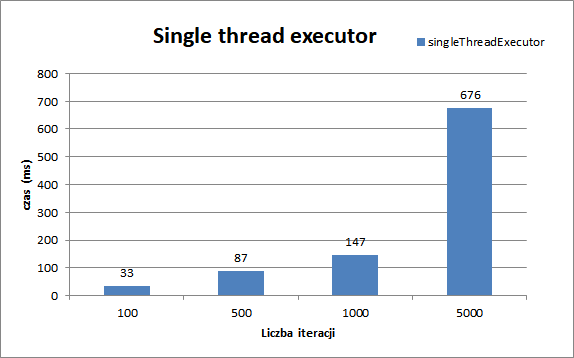
\includegraphics{s1.png}
    \captionof{figure}{Wyniki dla SingleThreadExecutor}
\end{center}

\begin{center}
\centering
    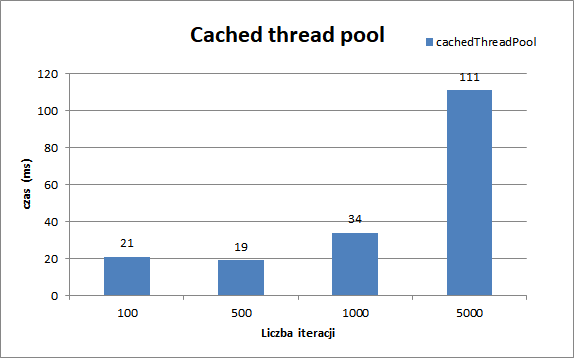
\includegraphics{c1.png}
    \captionof{figure}{Wyniki dla CachedThreadPool}
\end{center}
\vspace{1cm}

\begin{center}
\centering
    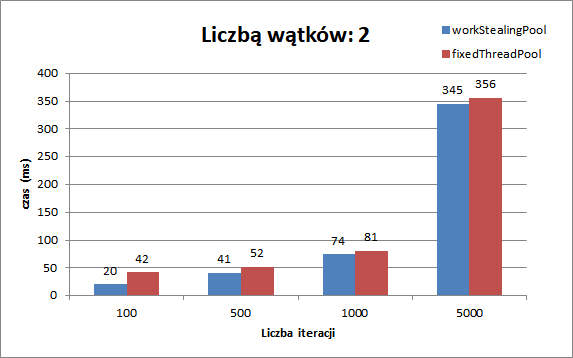
\includegraphics{compare1.png}
    \captionof{figure}{Porównanie fixedThreadPool z workStealingPool dla dwóch wątków}
\end{center}

\begin{center}
\centering
    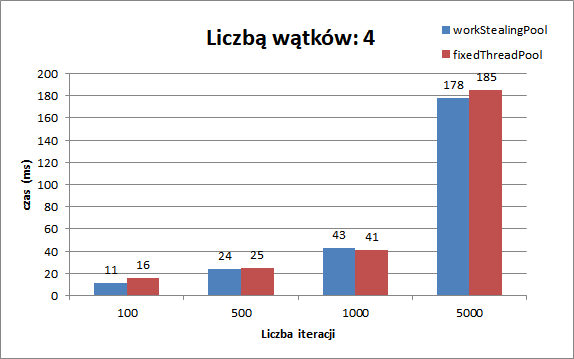
\includegraphics{compare2.png}
    \captionof{figure}{Porównanie fixedThreadPool z workStealingPool dla czterech wątków}
\end{center}
\vspace{1cm}

\begin{center}
\centering
    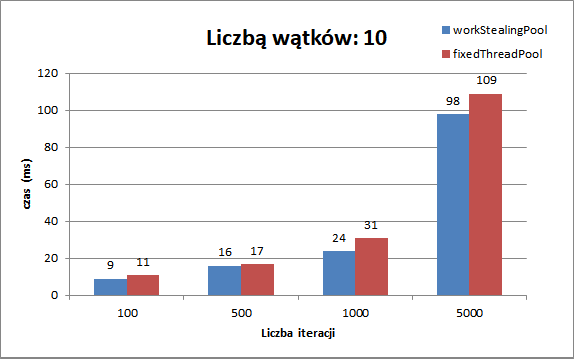
\includegraphics{compare3.png}
    \captionof{figure}{Porównanie fixedThreadPool z workStealingPool dla dziesięciu wątków}
\end{center}

\begin{center}
\centering
    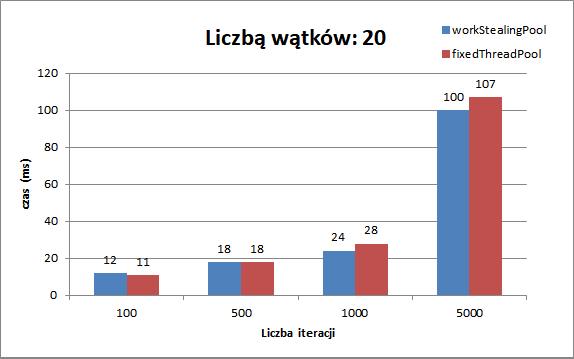
\includegraphics{compare4.png}
    \captionof{figure}{Porównanie fixedThreadPool z workStealingPool dla dwudziestu wątków}
\end{center}

\section{Wnioski}
Obserwując powyższe wykresy, nasuwa się prosty wniosek - im większy parametr MAX\_ITERS, tym więcej czasu zajmują obliczenia. Można pokusić się o wniosek, że czas rośnie proporcjonalnie do liczby iteracji.

\medskip
\emph{Single Thread Executor} to \emph{Executor}, który do wykonywania obliczeń używa tylko jednego wątku. Zadania są wykonywane sekwencyjnie. O ile w przypadku małej liczby obliczeń jest to nie jest to podejście najgorsze, to gdy mamy do czynienia z większą ilością zadań, może okazać się, że ten typ \emph{Executora} jest korzystniejsza.

\medskip
Kolejnym typem \emph{Executora} jest \emph{Cached Thread Pool}. Ten typ charakteryzuje się tym, że używa ponownie wątków, jeśli takowe zakończyły już prace i są dostępne. W razie potrzeby (gdy nie ma dostępnych wolnych wątków, a jest nowe zadanie do wykonania) tworzy nowy wątek i przydziela mu zadanie. Wątki, które nie były długo używane (domyślnie 60 sekund) zostają usunięte z puli.
Porównując wykresy 2. oraz 3. widzimy znaczną poprawę szybkości działania. Największy zysk (ponad sześciokrotny) można zauważyć gdy liczba iteracji wynosiła 5000. W tym przypadku zrównoleglenie obliczeń dało bardzo dobre rezultaty.

\medskip
Na ostatnich czterech wykresach zostały porównane \emph{Fixed Thread Pool Executor} oraz \emph{Work Stealing Pool Executor}. W pierwszej implementacji mamy do czynienia ze stałą pulą wątków, które przyjmują kolejne zadania do wykonania. Natomiast drugi wariant jest nieco bardziej skomplikowany. \emph{Work Stealing Pool Executor} polega na dzieleniu zadania na mniejsze podzadania, jeśli jest ono dość skomplikowane. Każdy wątek oblicza jakąś część podproblemu, a gdy już wszystkie części zostaną obliczone, to części zostają połączone ze sobą w jedną całość (lub nie, jeśli zadanie nie polega na zwracaniu czegoś, a jedynie na obliczeniach). Warto dodać, że ten typ \emph{Executora} nie gwarantuje w żaden sposób kolejności wykonywania kolejnych zadań. Problem wyliczania zbioru Mandelbrota nie jest typem problemu, w którym każde podzadanie (obliczenie wartości pikseli kolejnych wierszy obrazu wynikowego) jest skomplikowane, więc potencjał tej metody nie został wykorzystany. Porównując czasy wykonań można zauważyć, że są bardzo zbliżone do siebie, różnice sięgają co najwyżej kilkunastu milisekund.
Inną kwestią wartą obserwacji jest fakt, że przy liczbie wątków równej 20, zysk nie jest tak duży, jakby się można było spodziewać. Może to wynikać z faktu, że testy były przeprowadzane na procesorze, który ma cztery rdzenie i obługuje osiem wątków, więc zysk wynikający ze zwiększania puli nie jest widoczny.

\medskip
Podsumowując, wzorzec \emph{Executor} potrafi znacznie uprościć tworzenie wielowątkowych programów, ponieważ programista nie musi implementować puli wątków. Dodatkowo, Java dostarcza różnych implementacji wzorca \emph{Executor} o ciekawych własnościach, co pozwala dodatkowo zoptymalizować użycie dostępnych zasobów sprzętowych. Samo zrównoleglanie operacji pozwala na znaczne przyspieszenie obliczeń, które nie zależą od poprzednich wyników. Wzorzec \emph{Future} jest bardzo wygodny w użyciu oraz pozwala, aby program kontynuował działanie po zleceniu zadania. Dzięki temu obliczenia mogą być prowadzone w tle, a główny program wykonuje dalsze operacje. Gdy chcemy skorzystać z danych w obiekcie \emph{Future} możemy dostać je od razu, poczekać, aż się pojawią lub sprawdzić czy są dostępne, co daje dużą dowolność w tworzeniu programu.

\newpage
\section{Bibliografia}
\begin{itemize}
    \item \url{https://docs.oracle.com/javase/7/docs/api/java/util/concurrent/Executors.html}
    \item \url{https://www.baeldung.com/java-executors-cached-fixed-threadpool}
    \item \url{https://www.baeldung.com/java-executor-service-tutorial}
    \item \url{https://docs.oracle.com/javase/8/docs/api/java/util/concurrent/Future.html}
    \item \url{https://docs.oracle.com/javase/8/docs/api/java/util/concurrent/Executors.html}
    \item \url{https://docs.oracle.com/javase/tutorial/essential/concurrency/executors.html}

\end{itemize}

\end{document}
